\documentclass[11pt]{article}

% Related to page geomety
\usepackage[a4paper,vmargin={2.4cm,2.8cm},hmargin={2.4cm,2.4cm}]{geometry}
\usepackage[utf8]{inputenc}
\usepackage{fancyhdr}
\pagestyle{fancy}
\renewcommand{\headrulewidth}{1pt}
\fancyhead[C]{CONFIDENTIAL}
\fancyhead[L]{Team 04 - Contour Detection}
\fancyhead[R]{M2DS Capstone projects, IPP, 2025}


% Related to math
\usepackage{amsmath,amssymb,amsfonts,amsthm}

% Related to figures
\usepackage{graphicx}

%Related to referencing
\usepackage{hyperref}
\usepackage{cleveref}

\begin{document}

\begin{center}
\textbf{Contour detection - mid-term checkpoint} \\
Fabien Lagnieu, Maha Kadraoui, Tristan Waddington, Abdoul Zeba\\
\textbf{Mentor:} Stéphane Maviel (CEO Vinci/Diane\footnote{Diane is Vinci's inside Startup tasked to find numerical solutions
to ease the work of Vinci collaborators.}) \\\vspace{2em}
\textbf{\Large }
\end{center}
\vspace{-1cm}
Architects are drawing floor plans using a CAD software. These files are used
by engineers to plan and conduct the construction of the building. In this process,
additional measures are needed such as the room size or adjacency. The goal of 
this project is to develop a tool that can automatically detect the contours of 
the rooms in the floor plan and draw it back in the CAD software. 

\begin{figure}[h]
    \centering
    
\includegraphics[width=0.1\textwidth]{figures/Diane.png}
    \hspace{0.2\textwidth}
    
\includegraphics[width=0.1\textwidth]{figures/ipparis.png}
    %\caption{Example figure with example spacing and caption: Left, ipp paris logo. Right, ipp paris logo.}
    \label{fig:my_label}
\end{figure}

\section{Context}
Vinci engineers are dealing with a different floor plan for every project they are working on.
Every plan has its own drawing style and the contours of the rooms are often mixed with other
lines, but they need this information to plan the location of smoke detectors, fire extinguishers,
and other facilities in the building. The goal of this project is to develop a tool that can
automatically detect the contours of the rooms in the floor plan and draw back the polygons in the CAD software as 
a vector layer for further automatic processing. 

Diane team already worked on this problem and developed a first version of the tool
that is too slow and not accurate enough. They are looking for other approaches
to improve it. They have shared with us 9 geojson exports of floor plans.

\section{Methods}
\label{sec:methods}
After a first phase of data cleaning we are focusing on two different paths to solve the problem:

\begin{enumerate}
    \item \textbf{Graph} Transform the list of lines into a graph and construct polygons \cite{Schafer2011AutomaticGO} then cluster the lines to create the polygons\cite{dominguez2012Semiautomaticdetection}.
    \item \textbf{CNNs} Using a dense literature review\cite{PIZARRO2022104348}, we 
    spotted some successful uses of CNNs\cite{ijgi10020097}. This same paper also provides the list
    of datasets of floor plans as image we can use.
\end{enumerate}

\section{Results}
The first experiments of clustering are not conclusive. The detection with 
CNN works well on well closed rooms but fails on open doors, see \cref{fig:CNN_results}.

\begin{figure}[htb!]
    \centering
    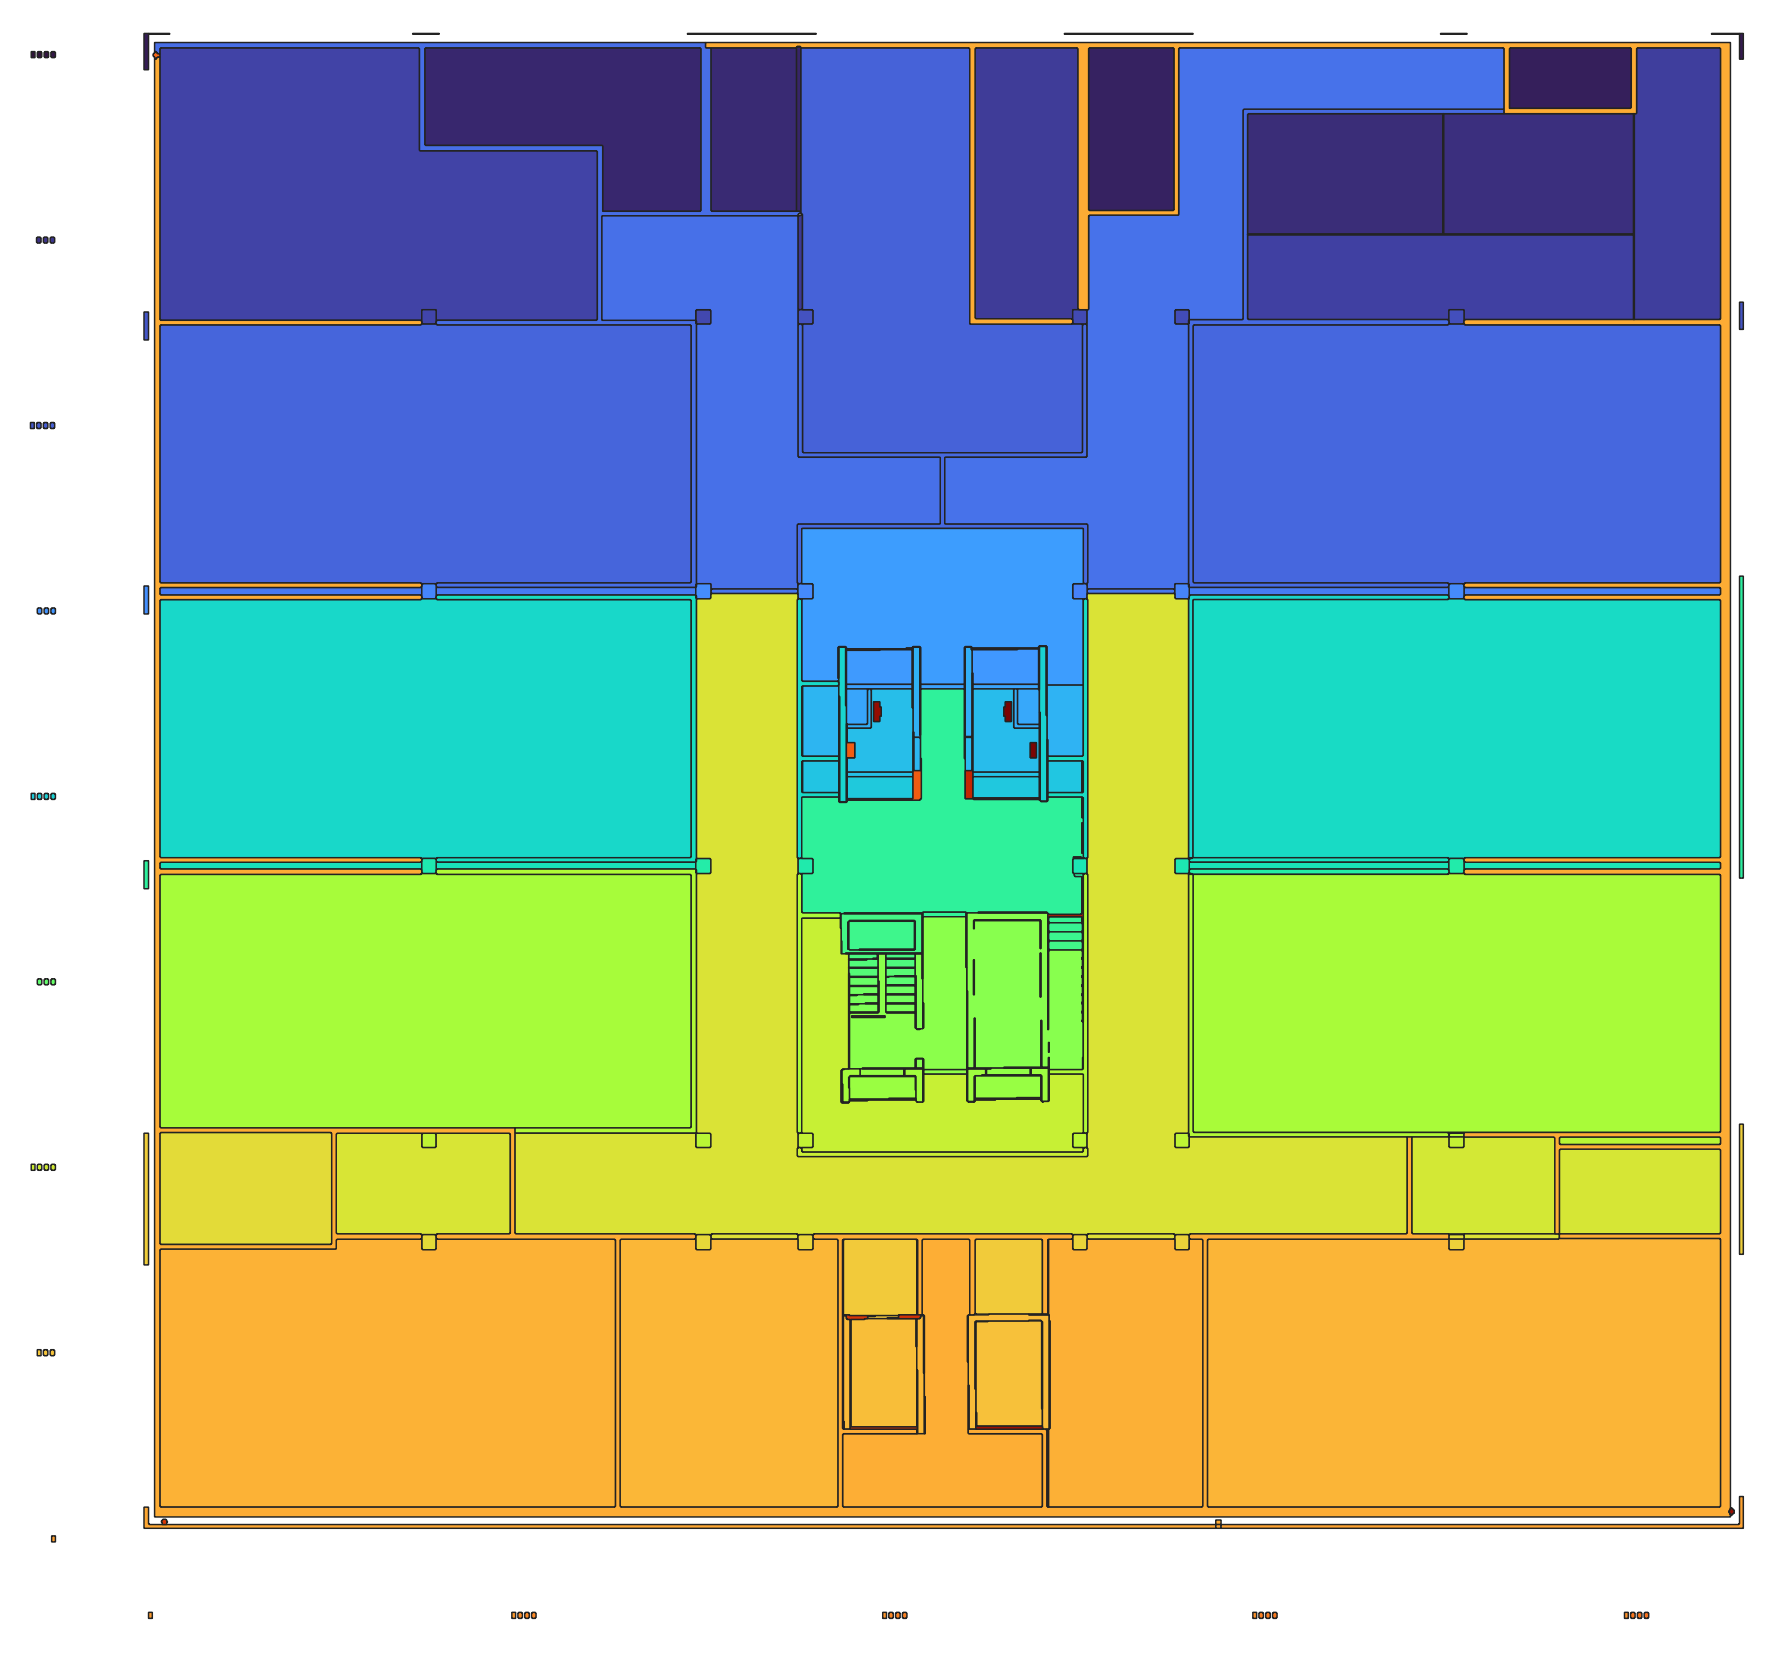
\includegraphics[width=0.4\textwidth]{figures/output4_CNN.png}
    %\hspace{0.2\textwidth}
    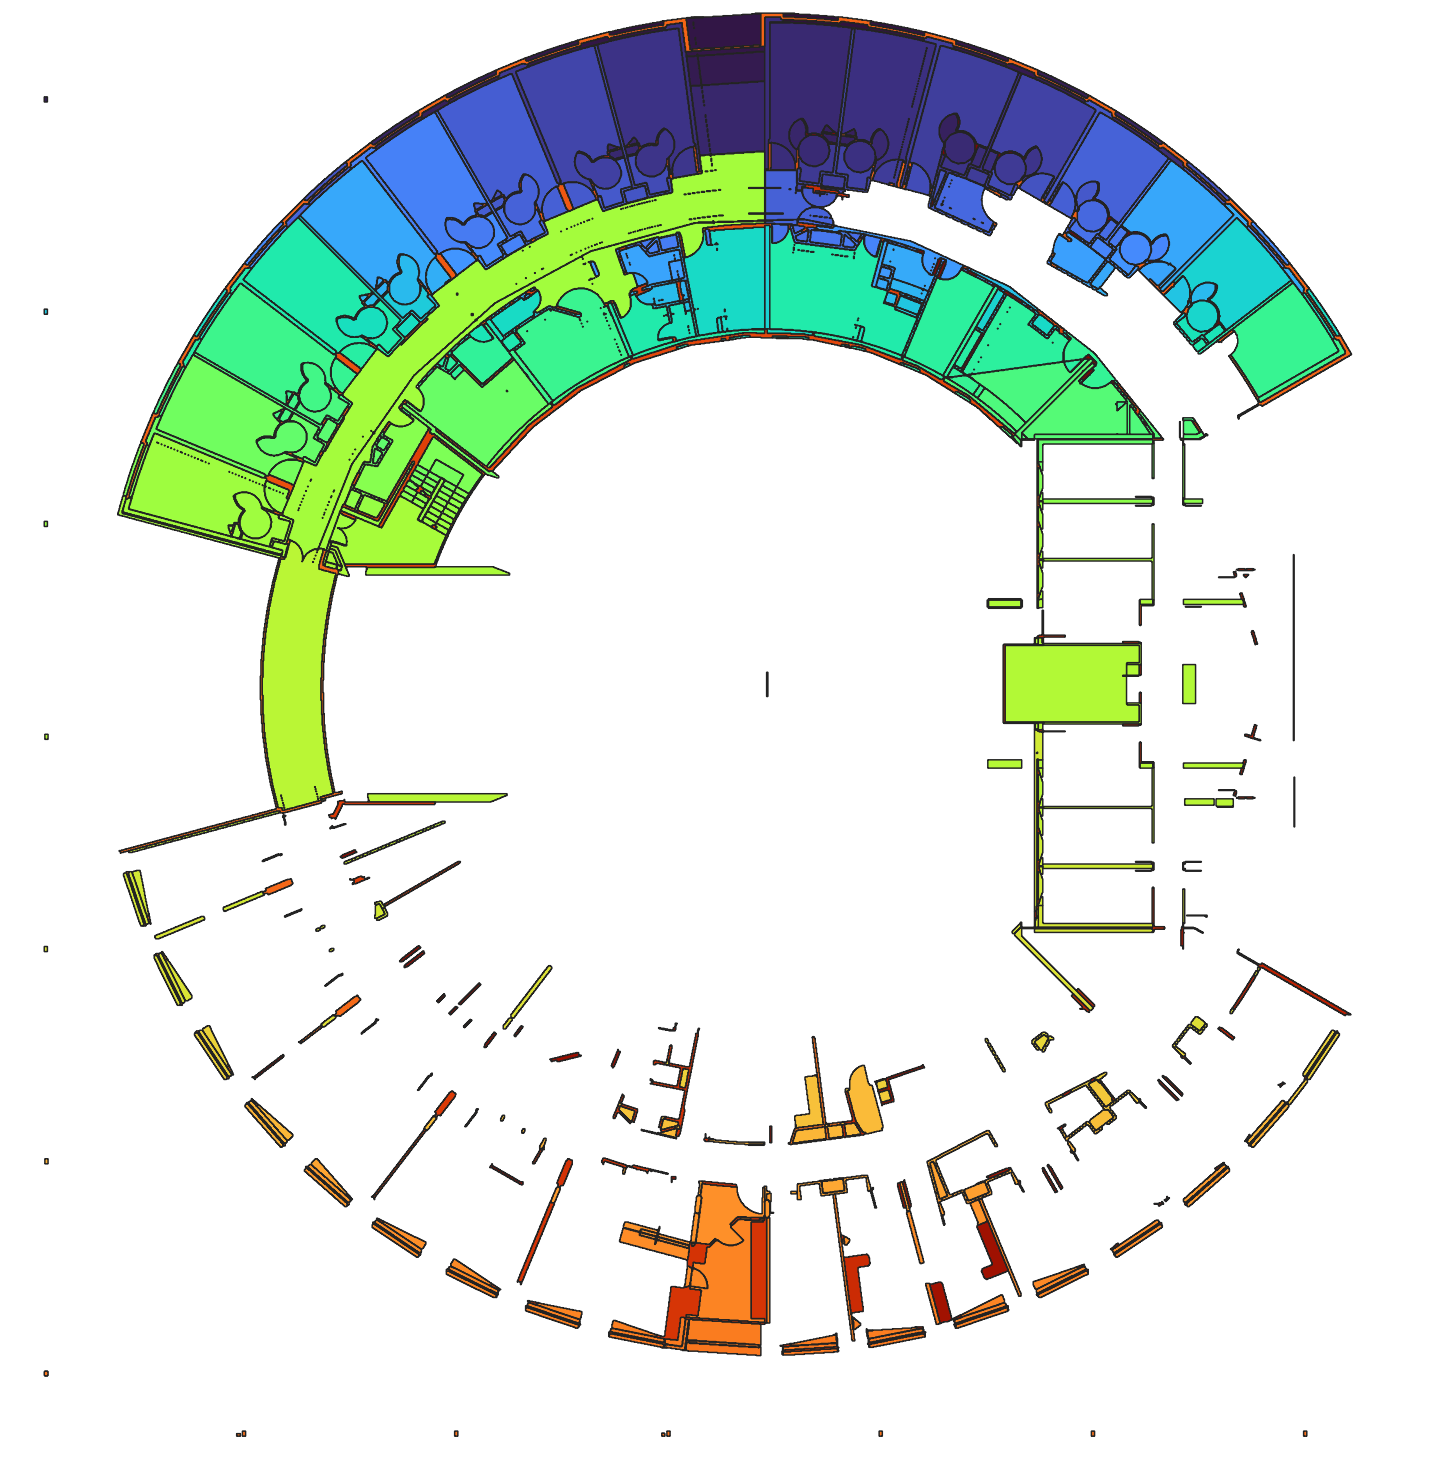
\includegraphics[width=0.4\textwidth]{figures/output7_CNN.png}
    \caption{Actual results of room detection with a CNN. Left: well closed rooms. Right, rooms with open doors are not detected.}
    \label{fig:CNN_results}
\end{figure}

\section{Conclusion}
Our main issue is that this project is not a machine learning problem. 
With less than 10 items to work on, they need a tailored solution on a very specific case with very high accuracy. This is highly challenging.

\paragraph{Organization within the team}
After a first diverging phase where every one has tried different methods, we are now focusing on the two paths described in \cref{sec:methods}. We are meeting every 
week to discuss our progress and share our results. We are also using a shared git repository to share our code and results\footnote{Private :https://github.com/waddason/CapstoneContour}.

\bibliographystyle{plain}
\bibliography{references}


\end{document}